\documentclass[12pt,twoside,draft]{book}
\usepackage{../../thesis}
\graphicspath{ {../../images/} }

\begin{document}

\chapter{Introduction}
In this chapter, I will introduce the logistic map as an example of a chaotic system, without defining what it means for a system to be ``chaotic''.
Next, I will discuss the origin of chaos.
At last, I discuss what ``chaos'' is.

\section{Our First Chaotic Map}

This is the equation for logistic map:
\begin{equation}
  L_{\mu}(x) = \mu x(1-x),
  \label{logistic}
\end{equation}
and the ``equivalent'' differential equation:
\begin{equation}
  \frac{dx}{dt} = \mu x(1-x)
  \label{logisticdiffeq}
\end{equation}
(In general, we can go between continuous and discrete models
\begin{align*}
  \frac{dx(t)}{dt} = G(x(t)) &\quad\mbox{(Continuous)} \\
  x(t + 1) = F(x(t)) &\quad\mbox{(Discrete)}
\end{align*}
by using the following approximation of the differential equation by mapping
\begin{equation*}
  \frac{dx(t)}{dt} \approx \frac{x(t_0 + (n+1)\Delta t) - x(t_0 + n \Delta t)}{\Delta t},
\end{equation*}
which leads to an approximation of the mapping by the differential equation
\begin{equation*}
  F(x(n)) \approx x(n) + \Delta t \cdot G(x(n))
\end{equation*}
.)
The only difference between equations \pref{logisticdiffeq} and \pref{logistic}

The differential equation \pref{logisticdiffeq} can be easily solved by separation of variables.
\begin{align*}
  \frac{dx}{x(1-x)} &= \mu dt \\  
  \left( \frac{1}{x} + \frac{1}{1-x} \right) dx &= \mu dt
\end{align*}
Then, suppose that $x(0) = x_0$, and integrate from $t = 0$ to $T$
\begin{align*}
  \int_{x_0}^{x(T)} \frac{1}{x} + \frac{1}{1-x} dx &= \int_0^T \mu dt \\
  \log{\frac{x(T)}{1-x(T)}} - \log{\frac{x_0}{1-x_0}} &= \mu T \\
  \frac{x(T)}{1-x(T)} &= \frac{x_0 e^{\mu T}}{1-x_0} \\
  (1-x_0)x(T) &= x_0 e^{\mu T} (1-x(T)) \\
  (1-x_0 + x_0 e^{\mu T})x(T) &= x_0 e^{\mu T}
\end{align*}

Thus, we have (with a slight change of notation)
\begin{equation}
  x(t) = \frac{x_0 e^{\mu t}}{1 - x_0 + x_0 e^{\mu t}}
  \label{eq:logisticdiffeqsoln}
\end{equation}

Change in the growth rate $\mu$ does not alter the bahaviour.
\begin{figure}[ht]
  \begin{center}
    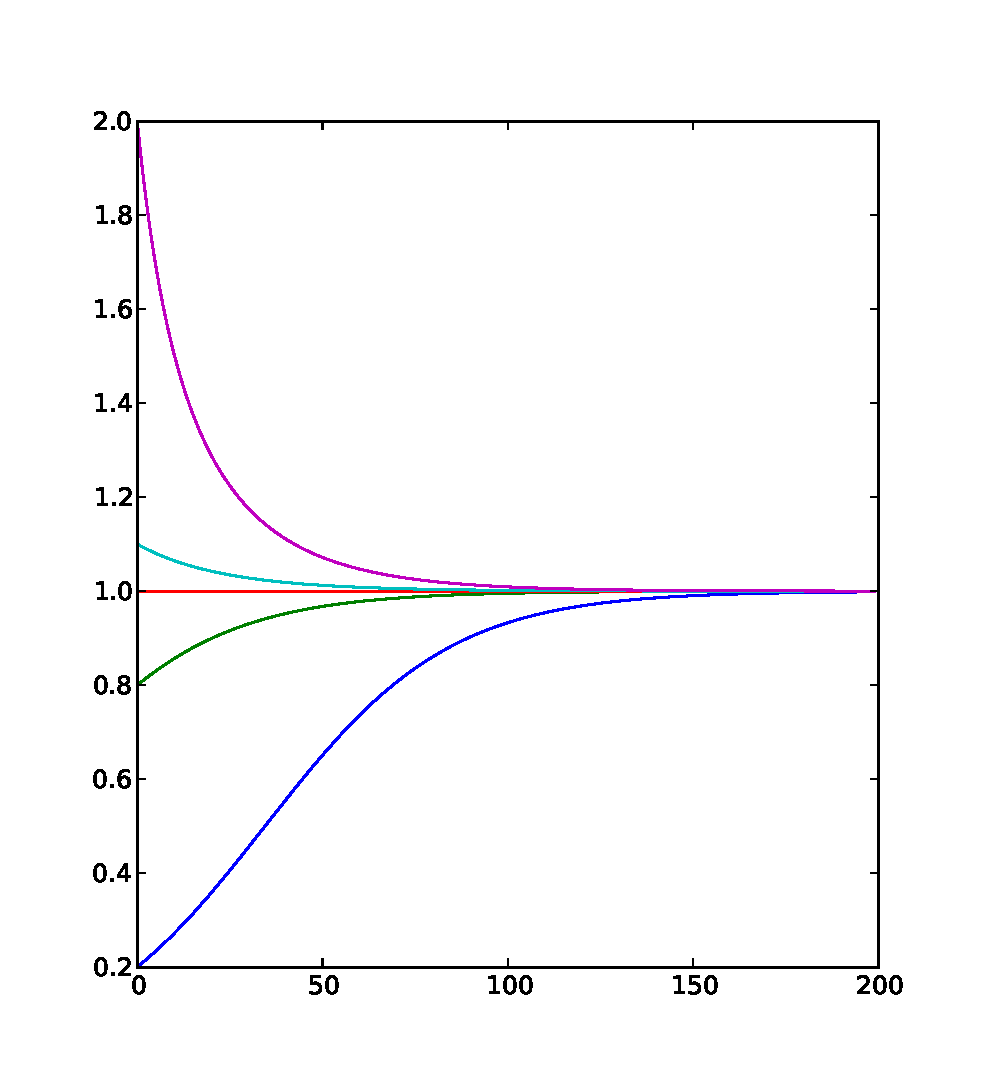
\includegraphics[scale=0.5]{logistic_diffeq_mu4_varyingx0}
  \end{center}
  \caption{
    Plot of equation \pref{eq:logisticdiffeqsoln} with $\mu = 4$ and various $x_0$. 
  Note that regardless of the initial value, $x(t)$ converges to $1$.
}
  \label{fig:logistic_diffeq1}
\end{figure}

%\begin{figure}[h]
%  \begin{center}
%    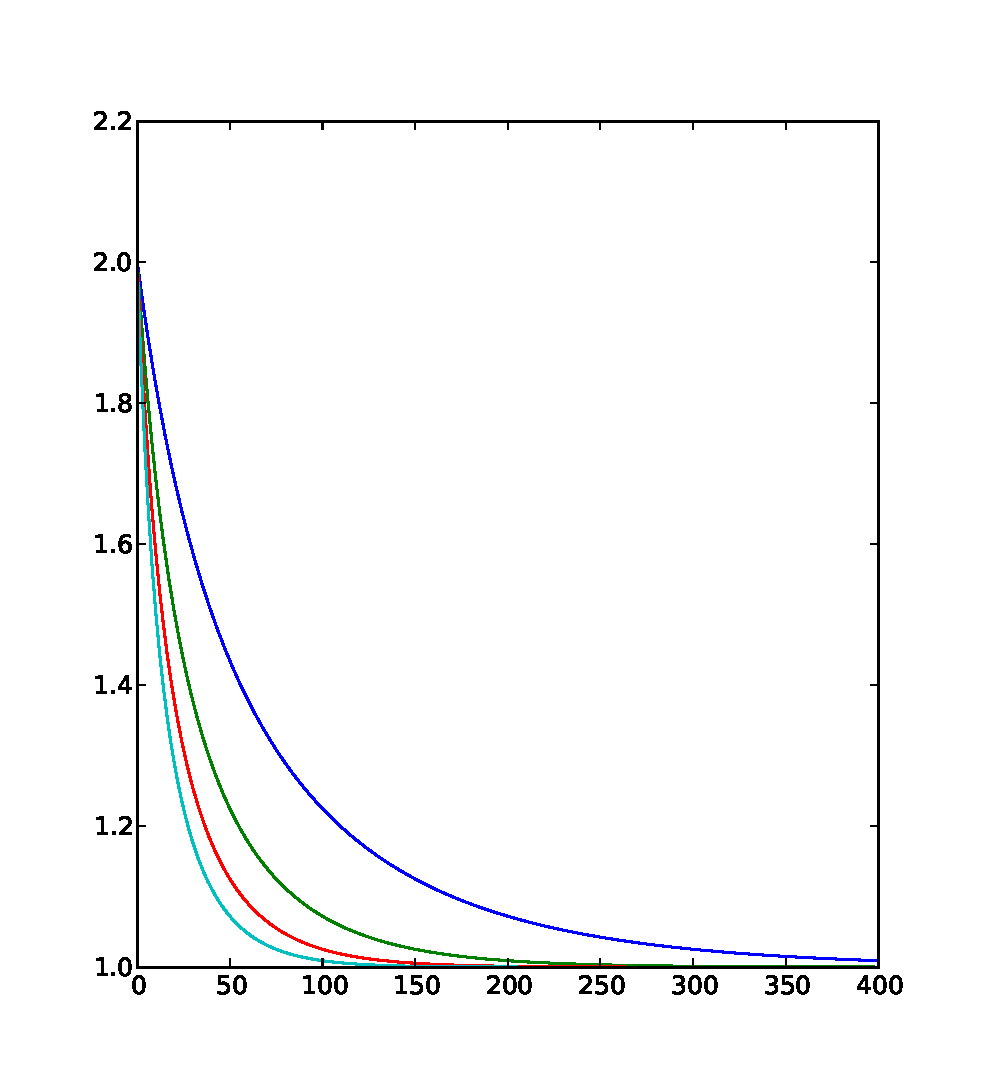
\includegraphics[scale=0.5]{logistic_diffeq_mu1234_x2}
%  \end{center}
%  \caption{
%    Plot of equation \pref{eq:logisticdiffeqsoln} with $x_0 = 2$ and various $\mu$ (1,2,3,4).
%    As $\mu$ increases, $x(t)$ converges to $1$ faster.
%    However, it does not alter the overall behaviour.
%  }
%  \label{fig:logistic_diffeq2}
%\end{figure}

\begin{figure}[h]
  \begin{center}
    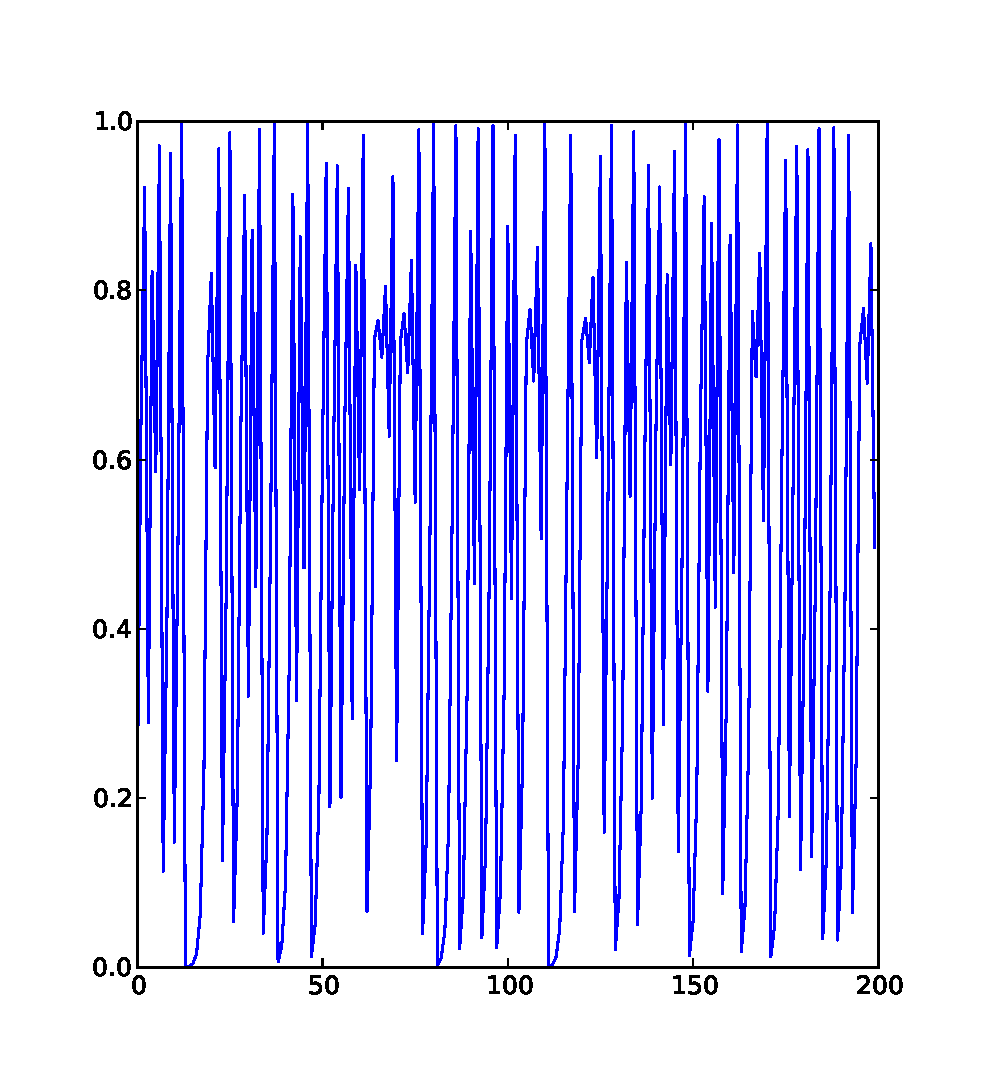
\includegraphics[scale=0.5]{logistic_map_mu4_x02}
  \end{center}
  \caption{
    Chaotic map.
  }
  \label{fig:logistic_map_chaotic}
\end{figure}


\section{The Origin of Chaos}
Edward Lorentz is often regarded as the first discoverer of chaos.
\begin{figure}[t]
  \begin{center}
    \includegraphics[scale=0.5]{golden_lorentz_attractor}
  \end{center}
  \caption{Lorentz Attractor}
  \label{fig:lorentz}
\end{figure}
He found chaotic behaviours through atmospheric simulations using twelve differential equations.
In his seminal article ``Deterministic Nonperiodic Flow'', Lorentz discusses the chaotic behavior of a system of three differential equations, which were reduced from the original twelve equations.
Yoshisuke Ueda, though lesser known, was also one of the first scientists to recognize chaotic behaviors
In 1961 (a sketch of the ``Japanese Attractor''), while Lorentz's paper was published in 1963.
David Ruelle, a prominent French chaos researcher, introduced Ueda in \citet{ruelle}.
\footnote{Doubtful of Ueda's result, Ueda's mentor did not allow publication of Ueda's result until 1970, seven years after the publication of ``Deterministic Nonperiodic Flow.''
Because of the strict hierarchical structure of the Japanese academia, the first author of Ueda's paper, ``On the Behavior of Self-Oscillatory Systems with External Force'', is his mentor.%\cite[p89]{sprott}
``He was the emperor of his laboratory, and yet outwardly he was a mild-mannered gentleman.
I believed at that time that his was the most feudalistic of any laboratory in the world, and the wall of his authority was impenetrable during his reign, and I still believe it.
But because of that, we were not swept away by worldly concerns and could concentrate on our research, being faithful to our own ideas.''
``After my report, at any rate, Prof. Urabe admonished me personally.
'What you saw was simply the essence of quasi-periodic oscillations,' he said.
'You are too young to make conceptual observations.'
% 君が見たのは単に概周期振動にすぎない。概念的な所見を述べるのは、若い君のやることじゃない。
% Your result is no more than an almost periodic oscillation. Don't form a selfish concept of steady states. \citep[p.141]{gleick} : from 'Random Phenomena Resulting from Nonlinearity in the System Described by Duffing's Equation' (1985) in its postscript
The existence of random oscillations (chaos) was so obvious in my mind, that the negative comment did not crush me.
Even so, I was deeply disappointed that no one understood it no matter how hard I tried to explain.\citep[p47]{ueda-abraham}
Ueda left the following remark: ``Chaos, though common phenomena in the nature, has been dismissed because of the difficulty to grasp its full notion.''\citep[p533]{gleick}
Either way, vigorous research activities on chaos only started in the 70's.}
The reason that I would like to discuss this scientist instead of Lorentz is not because he is the first scientist to see chaos.
The name ``Japanese Attractor'' was given by David Ruelle.(Les assracteurs etranges; Strange Attractors, 1980)
% Ueda: 最初はアナログコンピュータが故障したのかと思った。しかしすぐに、いやそんなことはないと悟った (in Chaos Avant-Garde?)
``I thought vaccum tubes were broken or something---a common issues with computers of those days.'' \citep{lorentzbook} %私はすぐに真空管が弱ったか何かの、よくあるコンピュータトラブルを疑ったが、修理を頼む前に、どこで間違いが起ったかだけでも調べてみることにした
``As I look back, I feel that after those long exhausting vigils in front of the analog computer, staring atits output, chaos had become a totally natural, everyday phenomenon in my mind.
People call chaos a new phenomenon, but it has always been around.
There's nothing new about it---only people did not notice it.''\cite[p27]{ueda-abraham}
%「カオス現象は、われわれが、日常、目にしているありふれた実在の自然現象であるにもかかわらず、その概念把握の困難さのために、かっては見過ごされてきた」
The true value in Ueda's findings lies in its settings.
While Lorentz's discovery of chaos was through computer simulation of a hypothetical model, Ueda's was through an analog computer, a physical, real-world system.
``analog computeres solve coupled nonlinear equations by mimicking a physical system.
The error properties of a particular digital integration scheme need not ever be considered.
Indeed, within the range of accuracy limited by the tolerance of the components, the unsystematic errors caused by the thermal fluctuations and electronic noise in an analog simulation can actually be useful; this is the case, for example, in qualitative studies of chaotic dynamical systems.
% Crutchfiled, Farmer, Huberman 'Fluctuations and simple chaotic dynamics'
% Crutchfield, Packard 'Symbolic dynamics of one dimensional maps: Entropies, finite precision, and noise'
Specifically, these fluctuations obliterate the detailed fine structure found in the mathematical description of chaos and thus effectively mimic the coarse-grained behavior that is observed in actual physical experiments in, for example, convecting fluids or nonlinear electronic circuits.
''\cite[p.383]{campbell}
Chaos in the nature is seen elsewhere:
Libchaber confirmed chaos via bifurcation in an experiment involving Helium.
Logistic map is used to model population dynamics.
Lorentz system was created as a simplified model for atmosphere.
NH3 lazer is known to show chaotic behavior \citep{kantz-schreiber}.
B-Z reaction

\section{So What Is Chaos, After All?}
We tend to label a dynamical systems as ``chaotic'' on an intuitive ground.
If the orbit looks (judged by our visual sense organ complex), the system is called chaotic.
In 1986, the Royal Society held an international conference on chaos and defined ``chaos'' as ``Stochastic behavior occurring in a deterministic system.'' \cite{stewart}
Two Russian physicists famously said "A strange attractor seems strange only to a stranger."
(Boris Chirikov, Felix Izrailev)\cite{lorentzbook}

``As an academic term, I do not find the word 'chaos' very appropriate.
But what shall we call it then?
My proposal has been 'randomly transitional phenomena''; I will explain this below.
The characteristics of chaos in a physical system can be summarized as follows:
- Random phenomena that occur in deterministic systems.
- Random phenomena whose short-term behavior is predictable.
- Random phenomena whose long-term behavior is unpredictable.
- Although the phenomena are irregular and unpredictable, chaos does have a definite structure.
The original meaning of chaos, I feel, is a ``total disorder and ultimate unpredictability.''
But as scientific terminology, the word ``chaos'' seems to overemphasize the unpredictability alone.
\ldots
Even so I have to use the word ``chaos'' here \ldots
It is a concise expression which has already filtered into people's minds, and therefore I have decided it is rather pointless to resist it.
\citep[24]{ueda-abraham}

% Li and Yorke's essay in Chaos Avant-Garde: on how chaos developed over a decade since Poincare (202)
``He [Robert May] adoped our [Li and Yorke] use of 'chaos' as a mathematical term, and \textit{Period three implies chaos} therefore began to attract considerable worldwide attention by his strong advocacy in talks and papers.
\ldots
As use of the word 'chaos' spread, it became a word people loved to hate: they didn't have a better word but didn't like chaos.''
\citep[205]{ueda-abraham}

Although there is no universally accepted definition of chaos, most experts would concur that chaos is the {\it aperiodic, long-term behavior of a bounded, deterministic system that exhibits sensitive dependence on initial conditions} (Sprott, p104)

Our goal is to find the sufficient conditions that give rise to complex orbit structures.

\section{``The'' Definition of Chaos}
The chapter aims to develop descriptive, intuitive notion of chaos, without involved mathematics.
We will let go of mathematical rigor for the time being.
Discussion of precise mathematical definitions of chaos starts the chapter after this one.
The present chapter should prepare the reader for such abstract definitions.

\section{Invariants}
``By symmetry we mean an invariance against change: something stays the same, in spite of some potentially consequential alteration.''
%
``The word \textit{symmetric} is of ancient Greek parentage and means well-proportioned, well-ordered--certainly nothing even remotely chaotic.
Yet, paradoxically, self-similarity, the topic of this tome, alone among all the symmetries gives birth to its very antithesis: \textit{chaos}, a state of utter confusion and disorder.''
\cite[p.xiii-xv]{schroeder}

In subsequent sections, we will discuss two invariants of dynamical systems: \textit{Lyapunov exponents} and \textit{fractal dimension}.
Why are we interested in invariants?

\citet[p.51]{kantz-schreiber}:
\begin{quotation}
Noise reduction means that one tries to decompose a time series into two components, one of which supposedly contains the signal and the other one contains random fluctuations.
Thus we always assume that the data can be thought of as an additive superposition of two different components which have to be distinguishable by some objective criterion.
The classical statistical tool for obtaining this distinction is the power spectrum.

Random noise has a flat, or at least a broad, spectrum, whereas periodic or quasi-periodic signals have sharp spectral lines.
After both components have been identified in the spectrum, a Wiener filter can be used to separate the time series accordingly.
This approach fails for deterministic chaotic dynamics because the output of such systems usually leads to broad band spectra itself and thus possesses spectral properties generally attributed to random noise.
Even if parts of the spectrum can be clearly associated with the signal, a separation into signal and noise fails for most parts of the frequency domain. Chaotic deterministic systems are of particular interest because the determinism yields an alternative criterion to distinguish the signal and the noise. 
\end{quotation}

The critical feature of the invariants is that they are not sensitive to initial conditions
or small perturbations of an orbit, while individual orbits of the system are exponentially
sensitive to such perturbations. \citep[p.1334]{abarbanel}

\begin{quote}
In the same way power spectrum with a sharp peak characterizes a linear system, invariants such as Lyapunov exponents, fractal dimension, and (KS or topological) entropy characterize nonlinear systems.
Each orbit is sensitive to initial conditions; however, these invariants are preserved under small perturbations, which are prevalent in real-life situations.
\end{quote}

``[B]road (Fourier) power spectrum is a first indication of chaotic behavior, though it alone does not characterize chaos''\citep[p.1338]{abarbanel}

``We say that motion on an attractor is chaotic if it displays sensitive dependence on initial conditions.'' \citep[p.11]{ott1994}
Two complementary attributes and quantifiers for these attributes sometimes used to define chaos are \citep[p.379]{abarbanel}, %this is not Ott!Abarbanel, then?
``[\ldots] two key aspects of chaos are the stretching of infinitesimal displacements and the complex orbit structure in the form of a vast variety of possible orbits.'' \citep[p.31]{ott1994}
\begin{enumerate}
  \item exponentially sensitive dependence: the largest Lyapunov exponent 
  \item complex orbit structure: entropy, (metric, topological, or others)
\end{enumerate}

Although Abarbanel does not include it in his list, an attractor with fractal dimension is a signature of a complex dynamics.
Note that a treatment of entropy--\textit{topological entropy}, to be specific--will be discussed in a later chapter with a more mathematical rigor.

\section{Geoetric Definition?}
I shall briefly describe a two-dimensional map called \textit{the baker's map}, which will facilitate our understandings of Lyapunov exponents and fractal dimension.
Also, the baker's map will be frequently used to illustrate definitions of chaos in later chapters.
Familiarity with this map would be helpful throughout the rest of the paper.

\begin{definition}
  Let $I = [0,1]$, and $0 \leq \alpha, \beta \leq 1$.
  The baker's map $B_{\alpha, \beta, \gamma, \delta}: \R^2 \to \R^2$ is defined as
  \begin{equation*}
    B_{\alpha, \beta, \gamma, \delta}(x,y) = (BX_{\alpha, \beta, \gamma, \delta}(x), BY_{\alpha, \beta, \gamma, \delta}(y)),
  \end{equation*}
  where
  \begin{equation*}
    BX_{\alpha, \beta, \gamma, \delta}(x) =
     \begin{cases}
      \alpha x  &\mbox{ for } y < \gamma \\
      (1 - \beta) + \beta x  &\mbox{ for } y \geq \gamma,
    \end{cases}
  \end{equation*}
  and
  \begin{equation*}
    BY_{\alpha, \beta, \gamma, \delta}(x) =
     \begin{cases}
       y/\gamma  &\mbox{ for } y < \gamma \\
       (y - \gamma)/ \delta  &\mbox{ for } y \geq \gamma.
    \end{cases}
  \end{equation*}

  \label{defn:baker}
  \index{baker's map}
\end{definition}

The name of the map comes from the way it operates on a square area.
It is stretching, squeezing, and folding that characterizes the baker's map.
And in fact--at least at an intuitive level--that is what produces chaos.
The best way to see how this simple map gives rise to the aforementioned characteristics of chaos--sensitive dependence on initial conditions and complex orbit structure--is to compute the transformation of $I \times I$ under iteration.

SHOW THE TRANSFORMATION

\section{Dimensions}
Definition of strange attractor\citep[p.131]{ruelle}

An example where the Hausdorff dimension has an advantage over the box-counting dimension.
Consider the following infinite sequence:
\begin{equation*}
  1, \frac{1}{2}, \frac{1}{3}, \frac{1}{4}, \cdots
\end{equation*}
The sequence, when regarded as a set on the real line, has a non-zero box-counting dimension.
It may be viewed as a dificiency of the box-counting dimension, as one expects that
a set of discrete points is zero-dimensional.
The Hausdorff dimension, however, yields zero for this set.

In the next two sections, we will prove that two nearby initial points are separated from each other exponentially fast by computing the Lyapunov exponent of the map, and show that the limit set of the map has a fractal dimension.
Also, the characteristics of the baker's map--streching, squeezing, and folding--turn out to be the primary means of providing mathematically rigorous definition of chaotic maps, as we will see in later chapters.
% Rossler: ``a sausage in a sausage in a sausage in a sausage'

(Order and Chaos p103)
Given that no precise scientific definition exists for the noun ``chaos'' or for the adjective ``chaotic,'' we will consider these words to be synonymous with certain typical properties.
We will say that a dynamical regime is chaotic if its power spectrum contains a continuous part---a broad band---regardless of the possible presence of peaks.
Or else we may use the criterion that the autocorrelation function of the time signal has finite support, i.e. that it goes to zero in a finite time.
In either case, the same concept is involved: the loss of memory of the signal with respect to itself.
Consequently, knowledge of the state of the system for an arbitrarily long time does not enable us to predict its later evolution.
Essentially, this means that we are making unpredictability the quality which defines chaos.
The characterization is pragmatic; it lacks rigor and contains unavoidable ambiguities.
The boundary separating predictability from unpredictability is unclear, leaving open questions such as:
- On what time scale must the flow be predictable?
- How precise must the prediction be?
- Can we allow a statistical prediction?
The distinction between the theoretical and practical impossibility of prediction is also problematic.
But given the current state of knowledge, it would be premature to try to do better.

\section{Lyapunov Exponents}
Positive Lyapunov exponent.\citet{kantz-schreiber} 
The technique of Lyapunov exponents was developed by Alexander M. Lyapunov to study stability of solutions for systems of differential equations.

Lyapunov exponents are sometimes called characteristic exponents.
Lai-Sang Young gave a lower bound of the Hausdorff dimension in terms of the Lyapunov numbers (log of Lyapunov exponents).


\subsection{In One Dimension}
\begin{definition}
  (Lyapunov number)
  Given a map $F$ and a $p-$periodic point $x_p$, the Lyapunov number of the point $N(x_p)$ is
  defined to be the spectral radius of the Jacobian matrix of the map.
  \begin{equation*}
    N(x_p) = \left[ \rho\left( F^p(x_p) \right) \right]^{1/p}
  \end{equation*}
  \label{def:lyapnum}
\end{definition}

\begin{definition}
  (Lyapunov Number, alternative)
  Let
  \begin{equation*}
    O(x_1) = \set{x_1, x_2, x_3, \ldots}
  \end{equation*}
  and define matrices
  \begin{equation*}
    A_1 = \frac{d}{dx}F(x_1),\; A_2 = \frac{d}{dx}F(x_2),\; \ldots,\; A_n = \frac{d}{dx}F(x_n).
  \end{equation*}
  Then consider their spectral radii
  \begin{equation*}
    \rho_1(x_1), \rho_2(x_1),\; \ldots,\; \rho_n(x_1).
  \end{equation*}
  Then the alternate version of the Lyapunov number $N(x_1)$ of $O(x_1)$ is defined as 
  \begin{equation*}
    N(x_1) = \lim\limits_{n \to \infty} (\rho_n(x_1))^{1/n}.
  \end{equation*}
\end{definition}
The alternative definition can be shown to be equivalent to the first definition.

Lyapunov exponent is computationally preferable to the Lyapunov number.
\begin{definition}
  (Lyapunov exponent)
  \begin{equation*}
    \Lambda(x_1) = \log N(x_1).
  \end{equation*}
  In particular,
  \begin{equation*}
    \Lambda(x_1) = \lim\limits_{n \to \infty} \paren*{\log\abs{F'(x_n)} + \log\abs{F'(x_{n-1})} + \cdots + \log\abs{F'(x_1)}}
  \end{equation*}
\end{definition}

In some cases, this yet another alternate definition is more convenient.
This version ignores transient states.
\begin{definition}
  (Lyapunov Number, yet another alternative)
  \begin{equation*}
    N(x_1, k) = N(x_k)
  \end{equation*}
  Then the Lyapunov number is defined to be
  \begin{equation*}
    N(x_1) = \lim\limits_{k \to \infty} N(x_1,k).
  \end{equation*}
\end{definition}

It can be shown that the Lyapunov exponent of a map is (almost everywhere) equivalent to the Lyapunov exponent of any orbit of a map (Lyapunov exponent is independent of orbit).

\subsection{Lyapunov Exponents and Conjugacy}
Lyapunov number of one-dimensional dynamical systems that are conjugate is the same
as long as $h'(x) \neq 0$ and
\begin{equation*}
  \lim\limits_{n\to \infty} \frac{\log\abs{h'(x_n)}}{n} = 0.
\end{equation*}

By the definition of conjugacy,
\begin{equation*}
  h'(x_{n+1})F'(x_n)\ldots F'(x_1) = G'(y_n)\ldots G'(y_1)h'(x_1).
\end{equation*}
Then 
\begin{align*}
  \Lambda(x_1) &= \lim\limits_{n\to \infty} \frac{1}{n}\paren{\log\abs{F'(x_n)} + \cdots + \log\abs{F'(x_n)} } \\
  &= \lim\limits_{n\to \infty} \frac{1}{n}\left(\log\abs{F'(x_n)} + \cdots + \log\abs{F'(x_n)} + \log\abs{h'(x_{n+1})}\right) \\
  &= \lim\limits_{n\to \infty} \frac{1}{n} \paren*{ \log\abs{G'(x_n)} + \cdots + \log\abs{G'(x_n)} + \log\abs{h'(x_1)} } \\
  &= \lim\limits_{n\to \infty} \frac{1}{n} \paren*{ \log\abs{G'(x_n)} + \cdots + \log\abs{G'(x_n)} } \\
  &= \Lambda(y_1),
\end{align*} 
as desired.

Although Lyapunov exponent is regarded as the standard method of distinguishing in the field of physics, we do not discuss it in detail, since Lyapunov exponent is a topic in differentiable dynamics, while our focus is on topolgical dynamics.
Even so, Lyapunov exponent should be treated with some care, as the next exmaple suggests.
\begin{example}
  \citep{wiggins}
  Consider the following vector field:
  \begin{equation*}
    \dot{x} = ax,
  \end{equation*}
  where $x \in \R$, and $a \in \R$ is a constant.
  The Lyapunov exponent of each orbit is $a > 0$.
\end{example}

\bibliographystyle{../../bibliography/pjgsm}
\bibliography{../../bibliography/thesis}

\end{document}
